%%%%%%%%%%%%%%%%%%%%%%%%%%%%%%%%%%%%%%%%%%%%%%%%%%%%%%%%%%%%%%%%%%%%%%%%%%%%%%%%%%
\begin{frame}[fragile]\frametitle{}

\begin{center}
{\Large Project: Sentiment Analysis of Movie Reviews}

(Ref: Sentiment Analysis using Tf-Idf weighting: Python/Scikit-learn, ML Bot 2 )
\end{center}
\end{frame}

%%%%%%%%%%%%%%%%%%%%%%%%%%%%%%%%%%%%%%%%%%%%%%%%%%%%%%%%%%%%%%%%%%%%%%%%%%%%%%%%%%
\begin{frame}[fragile]\frametitle{Objective}
  \begin{itemize}
  \item Sentiment analysis in text mining is the process of categorizing opinions expressed in a piece of text. 
  \item A basic form of such analysis would be to predict whether the opinion about something is positive or negative (polarity). 
  \item Our objective : To do sentiment polarity analysis on movie reviews.
  \end{itemize}
\end{frame}

%%%%%%%%%%%%%%%%%%%%%%%%%%%%%%%%%%%%%%%%%%%%%%%%%%%%%%%%%%%%%%%%%%%%%%%%%%%%%%%%%%
\begin{frame}[fragile]\frametitle{Dataset}
  \begin{itemize}
  \item Polarity Dataset: https://www.cs.cornell.edu/people/pabo/movie-review-data/review\_polarity.tar.gz
  \item 2000 labelled files of movie reviews with 1000 files for each of the two sentiments.
  \item We have to train a classifier based on some feature of the sentiment classes
  \end{itemize}
    \begin{lstlisting}  
  #Create a corpus with each document having one string
root_dir = 'txt_sentoken'
corpus = make_Corpus(root_dir)
    \end{lstlisting}
\end{frame}

%%%%%%%%%%%%%%%%%%%%%%%%%%%%%%%%%%%%%%%%%%%%%%%%%%%%%%%%%%%%%%%%%%%%%%%%%%%%%%%%%%
\begin{frame}[fragile]\frametitle{Dataset: Corpus}
    \begin{lstlisting}
def make_Corpus(root_dir):
    polarity_dirs = [os.path.join(root_dir,f) for f in os.listdir(root_dir)]    
    corpus = []    
    for polarity_dir in polarity_dirs:
        reviews = [os.path.join(polarity_dir,f) for f in os.listdir(polarity_dir)]
        for review in reviews:
            doc_string = "";
            with open(review) as rev:
                for line in rev:
                    doc_string = doc_string + line
            if not corpus:
                corpus = [doc_string]
            else:
                corpus.append(doc_string)
    return corpus
    \end{lstlisting}
\end{frame}

%%%%%%%%%%%%%%%%%%%%%%%%%%%%%%%%%%%%%%%%%%%%%%%%%%%%%%%%%%%%%%%%%%%%%%%%%%%%%%%%%%
\begin{frame}[fragile]\frametitle{Dataset Labels}
Known labels.
    \begin{lstlisting}
labels = np.zeros(2000);
labels[0:1000]=0;
labels[1000:2000]=1; 
    \end{lstlisting}
\end{frame}
        

%%%%%%%%%%%%%%%%%%%%%%%%%%%%%%%%%%%%%%%%%%%%%%%%%%%%%%%%%%%%%%%%%%%%%%%%%%%%%%%%%%
\begin{frame}[fragile]\frametitle{Dataset Split}
    \begin{lstlisting}
kf = StratifiedKFold(n_splits=10)
for train_index, test_index in kf.split(corpus,labels):
    X_train = [corpus[i] for i in train_index]
    X_test = [corpus[i] for i in test_index]
    y_train, y_test = labels[train_index], labels[test_index]
    \end{lstlisting}
   \begin{itemize}
  \item  From these 10 parts, 1 part is used for testing the model while the other 9 parts for training. 
  \item The validation process is repeated K times so that each of the partition is validated at least once without getting included in training set.
    \end{itemize}
\end{frame}

%%%%%%%%%%%%%%%%%%%%%%%%%%%%%%%%%%%%%%%%%%%%%%%%%%%%%%%%%%%%%%%%%%%%%%%%%%%%%%%%%%
\begin{frame}[fragile]\frametitle{Features and Classifier}
  \begin{itemize}
  \item We will be focusing mainly on the most popular and widely used word weighing scheme in text mining problems, known as term frequency and inverse document frequency (tf-idf) . 
  \item Further, we will be training a Support Vector Machine(SVM) classifier and Multinomial Naive Bayes classifier on tf-idf weighted word frequency features. 
  \item Finally, we will analyse the effect of using this scheme while checking the performance of the trained model on test movie reviews files.
  \end{itemize}
\end{frame}

%%%%%%%%%%%%%%%%%%%%%%%%%%%%%%%%%%%%%%%%%%%%%%%%%%%%%%%%%%%%%%%%%%%%%%%%%%%%%%%%%%
\begin{frame}[fragile]\frametitle{Tf-Idf weighted Word Count Feature Extraction}
  \begin{itemize}
  \item TF: Term Frequency: $tf(t,d) = F(t,d)$, where where $F(t,d)$ is number of occurrences of term $t$ in document $d$. 
  \item Pragamtically, log is taken to scale it properly $tf(t,d) = log(F(t,d))$
  \item IDF: Inverse Document Freqeuncy: $idf(t,D) = log(N/N_{t \in d})$, Here, $N$ is the total number of files in the corpus $D$ and $N_{t \in d}$ is number of files in which term $t$ is present. 
  \item Basically, the rare keywords get special treatment and stop words/non-distinguishing words get punished
  \item For each term in a file, $tf-idf(t,d,D) = tf(t,d) . idf(t,D)$
  \end{itemize}
\end{frame}

%%%%%%%%%%%%%%%%%%%%%%%%%%%%%%%%%%%%%%%%%%%%%%%%%%%%%%%%%%%%%%%%%%%%%%%%%%%%%%%%%%
\begin{frame}[fragile]\frametitle{Tf-Idf weighted Word Count Feature Extraction}
  \begin{itemize}
  \item We will divide the corpus in 90:10 split so that 1800 review files will be utilized as training set and rest 200 review files as test set. 
  \item The below code snippet shows how to extract features from the text files.
  \end{itemize}
    \begin{lstlisting}
vectorizer = TfidfVectorizer(min_df=5, max_df = 0.8, sublinear_tf=True, use_idf =True, stop_words = 'english')
train_corpus_tf_idf = vectorizer.fit_transform(X_train)
test_corpus_tf_idf = vectorizer.transform(X_test)
  \end{lstlisting}
\end{frame}

%%%%%%%%%%%%%%%%%%%%%%%%%%%%%%%%%%%%%%%%%%%%%%%%%%%%%%%%%%%%%%%%%%%%%%%%%%%%%%%%%%
\begin{frame}[fragile]\frametitle{Tf-Idf weighted Word Count Feature Extraction}
Sample tfidf Doc Term Matrix
    \begin{lstlisting}
  (0, 8108)	0.0277593819403
  (0, 10901)	0.141371596276
  :	:
  (1799, 9297)	0.0914125148715
  (1799, 12020)	0.0981878064009
  \end{lstlisting}
  (Doc Id, Term Id, tfidf score)
    \begin{center}
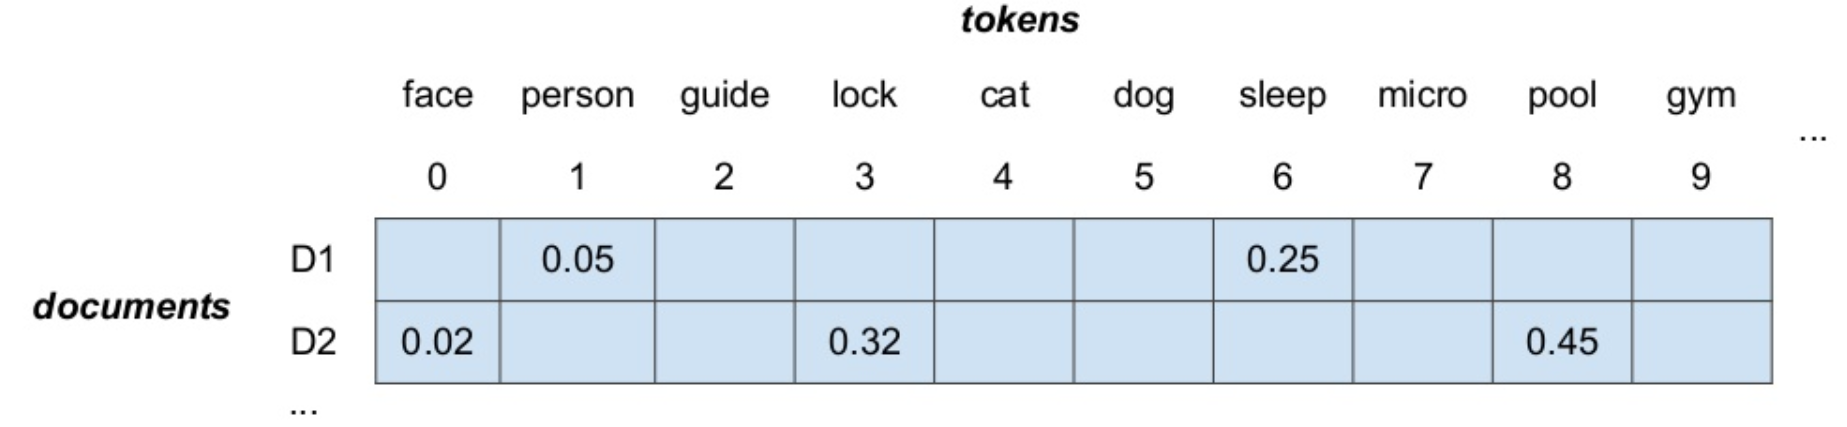
\includegraphics[width=\linewidth,keepaspectratio]{tfidfdocterm}
\end{center}
\end{frame}

        

%%%%%%%%%%%%%%%%%%%%%%%%%%%%%%%%%%%%%%%%%%%%%%%%%%%%%%%%%%%%%%%%%%%%%%%%%%%%%%%%%%
\begin{frame}[fragile]\frametitle{Tf-Idf weighted Word Count Feature Extraction}
  \begin{itemize}
  \item  min\_df : remove the words from the vocabulary which have occurred in less than `min\_df' number of files.
  \item      max\_df : remove the words from the vocabulary which have occurred in more than `max\_df' * total number of files in corpus.
  \item      sublinear\_tf : scale the term frequency in logarithmic scale.(talked about this earlier).
  \item      stop\_words : remove the predefined stop words of that language if present.
  \item      use\_idf : weight factor must use inverse document frequency(obviously).
%  \item      token\_pattern : It is a regular expression for the kind of words chosen in vocabulary. default: u'(?u)\b\w\w+\b' which means words only with 2 or more alphanumeric characters. If you want to keep only words with 2 or more alphabets(no numeric) then set token\_pattern as ur'(?u)\b[^\W\d][^\W\d]+\b'  
%  \item      max\_features : choose maximum number of words to be kept in vocabulary ordered by term frequency.
%   \item vocabulary : If you have created your own vocabulary, give it as a list here otherwise it will generate vocabulary from the training data.

  \end{itemize}
\end{frame}


%%%%%%%%%%%%%%%%%%%%%%%%%%%%%%%%%%%%%%%%%%%%%%%%%%%%%%%%%%%%%%%%%%%%%%%%%%%%%%%%%%
\begin{frame}[fragile]\frametitle{Tf-Idf weighted Word Count Feature Extraction}
fit\_transform(X\_train) does the following things:
  \begin{itemize}
  \item  Tokenizes each of sentence, preprocesses it for removing special characters, stop words etc. 
\item Creates a vocabulary of words with count in training set. %Takes max\_features, min_df and max_df in consideration.
\item It returns a feature vectors matrix having a fixed length tf-idf weighted word count feature for each document in training set. 
\item This is also called term-document matrix.
  \end{itemize}
\end{frame}

%%%%%%%%%%%%%%%%%%%%%%%%%%%%%%%%%%%%%%%%%%%%%%%%%%%%%%%%%%%%%%%%%%%%%%%%%%%%%%%%%%
\begin{frame}[fragile]\frametitle{Model}
  \begin{itemize}
  \item  Classifiers take two parameters, namely term-document matrix and polarity labels of the 1800 training files(900 positive and 900 negative). 
  \item  Similarly, vectorizer.transform(X\_test) will generate a term document matrix for the 200 test files using the same vocabulary generated while training. 
  \item We can check the performance of our trained models on the term document matrix of test set. 
  \end{itemize}
\end{frame}


%%%%%%%%%%%%%%%%%%%%%%%%%%%%%%%%%%%%%%%%%%%%%%%%%%%%%%%%%%%%%%%%%%%%%%%%%%%%%%%%%%
\begin{frame}[fragile]\frametitle{Model}
    \begin{lstlisting}
    model1 = LinearSVC()
    model2 = MultinomialNB()    
    model1.fit(train_corpus_tf_idf,y_train)
    model2.fit(train_corpus_tf_idf,y_train)
    result1 = model1.predict(test_corpus_tf_idf)
    result2 = model2.predict(test_corpus_tf_idf)
    \end{lstlisting}
\end{frame}

%%%%%%%%%%%%%%%%%%%%%%%%%%%%%%%%%%%%%%%%%%%%%%%%%%%%%%%%%%%%%%%%%%%%%%%%%%%%%%%%%%
\begin{frame}[fragile]\frametitle{Results}
    \begin{lstlisting}
    totalMatSvm = totalMatSvm + confusion_matrix(y_test, result1)
    totalMatNB = totalMatNB + confusion_matrix(y_test, result2)
    totalsvm = totalsvm+sum(y_test==result1)
    totalNB = totalNB+sum(y_test==result2)
    
# Accuracy
print(totalMatSvm)
print(totalMatNB)

# Confusion Matrix
print(totalsvm / 2000.0)
print(totalNB / 2000.0)
    \end{lstlisting}
\end{frame}

%%%%%%%%%%%%%%%%%%%%%%%%%%%%%%%%%%%%%%%%%%%%%%%%%%%%%%%%%%%%%%%%%%%%%%%%%%%%%%%%%%
\begin{frame}[fragile]\frametitle{Results}
    \begin{lstlisting}
0.874

0.8325
    \end{lstlisting}
 SVM outperforms Multinomial NB when using tf-idf weighted features
\end{frame}

%%%%%%%%%%%%%%%%%%%%%%%%%%%%%%%%%%%%%%%%%%%%%%%%%%%%%%%%%%%%%%%%%%%%%%%%%%%%%%%%%%
\begin{frame}[fragile]\frametitle{Results}
    \begin{lstlisting}
[[ 874.  126.]
 [ 126.  874.]]
 
[[ 856.  144.]
 [ 191.  809.]]
    \end{lstlisting}
Confusion matrix for both Multinomial NB and SVM using tf-idf features are shown below:
  \begin{center}
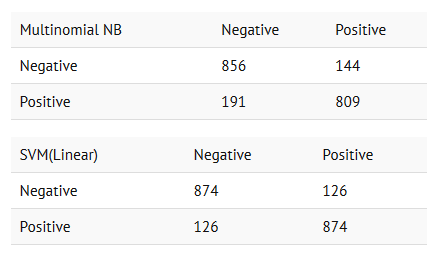
\includegraphics[width=0.5\linewidth,keepaspectratio]{tfidfsent}
\end{center}
\end{frame}

